\documentclass[12pt,a4paper]{article}
\usepackage[margin=1in]{geometry}
\usepackage{graphicx}
\usepackage{amsmath}
\usepackage{amssymb}
\usepackage{booktabs}
\usepackage{listings}
\usepackage{xcolor}
\usepackage{hyperref}
\usepackage{tikz}
\usetikzlibrary{shapes,arrows,positioning,calc}
\usepackage{float}
\usepackage{caption}
\usepackage{subcaption}

% Code listing style
\lstdefinestyle{verilog}{
    language=Verilog,
    basicstyle=\ttfamily\small,
    keywordstyle=\color{blue}\bfseries,
    commentstyle=\color{green!60!black},
    stringstyle=\color{red},
    numbers=left,
    numberstyle=\tiny\color{gray},
    numbersep=5pt,
    breaklines=true,
    frame=single,
    backgroundcolor=\color{gray!10},
    tabsize=4
}

\title{\textbf{4-Way Set-Associative Cache Design}\\
\large With Random Replacement Policy and Non-Blocking MSHR\\[1em]
\normalsize Hardware Design Project Report}

\author{Cache Memory Implementation for FPGA}
\date{December 2025}

\begin{document}

\maketitle

\begin{abstract}
This report presents the design and implementation of a 4-way set-associative cache memory with random replacement policy and non-blocking miss handling using Miss Status Holding Register (MSHR). The cache is implemented in Verilog HDL and targets the DE0-Nano FPGA board with Cyclone IV EP4CE22 device. The design features write-back policy with dirty bits, support for byte/half-word/word access, and comprehensive verification through simulation testbenches demonstrating cache hit latency, miss penalty, conflict misses, and write-back operations.
\end{abstract}

\tableofcontents
\newpage

%==============================================================================
\section{Introduction}
%==============================================================================

Cache memory is a critical component in modern computer architecture that bridges the speed gap between fast processors and slower main memory. This project implements a 4-way set-associative cache with the following key features:

\begin{itemize}
    \item \textbf{Organization}: 4-way set-associative
    \item \textbf{Replacement Policy}: Random (LFSR-based)
    \item \textbf{Write Policy}: Write-back with dirty bits
    \item \textbf{Miss Handling}: Non-blocking with MSHR
    \item \textbf{Data Access}: Byte, half-word, and word granularity
\end{itemize}

%==============================================================================
\section{Cache Architecture}
%==============================================================================

\subsection{Design Specifications}

The cache is designed with scalable parameters to support different sizes. The current implementation uses a 1KB configuration for fast synthesis:

\begin{table}[H]
\centering
\caption{Cache Configuration Parameters}
\begin{tabular}{@{}lll@{}}
\toprule
\textbf{Parameter} & \textbf{Value} & \textbf{Description} \\
\midrule
Cache Size & 1 KB & Total cache capacity \\
Number of Sets & 8 & Cache sets \\
Associativity & 4-way & Lines per set \\
Line Size & 32 bytes & Data per cache line \\
Total Lines & 32 & NUM\_SETS $\times$ ASSOC \\
Address Width & 20 bits & 1 MB addressable memory \\
Tag Bits & 12 bits & For address matching \\
Set Index Bits & 3 bits & $\log_2(8)$ \\
Offset Bits & 5 bits & $\log_2(32)$ \\
\bottomrule
\end{tabular}
\end{table}

\subsection{Address Breakdown}

For a 20-bit address accessing 1MB of memory:

\begin{figure}[H]
\centering
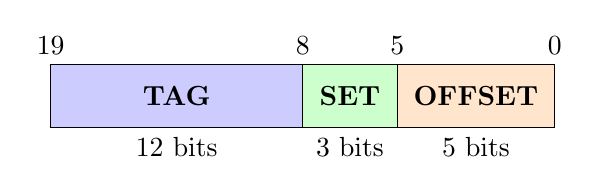
\begin{tikzpicture}[scale=0.8]
    % Address fields
    \draw[fill=blue!20] (0,0) rectangle (4,1);
    \draw[fill=green!20] (4,0) rectangle (5.5,1);
    \draw[fill=orange!20] (5.5,0) rectangle (8,1);
    
    % Labels inside
    \node at (2,0.5) {\textbf{TAG}};
    \node at (4.75,0.5) {\textbf{SET}};
    \node at (6.75,0.5) {\textbf{OFFSET}};
    
    % Bit positions
    \node[above] at (0,1) {19};
    \node[above] at (4,1) {8};
    \node[above] at (5.5,1) {5};
    \node[above] at (8,1) {0};
    
    % Bit widths below
    \node[below] at (2,0) {12 bits};
    \node[below] at (4.75,0) {3 bits};
    \node[below] at (6.75,0) {5 bits};
\end{tikzpicture}
\caption{20-bit Address Format for 1KB Cache}
\end{figure}

The address is decoded as follows:
\begin{align}
\text{Tag} &= \text{addr}[19:8] \quad \text{(12 bits)} \\
\text{Set Index} &= \text{addr}[7:5] \quad \text{(3 bits)} \\
\text{Block Offset} &= \text{addr}[4:0] \quad \text{(5 bits)} \\
\text{Word Offset} &= \text{addr}[4:2] \quad \text{(3 bits for word selection)}
\end{align}

\subsection{Cache Organization Diagram}

\begin{figure}[H]
\centering
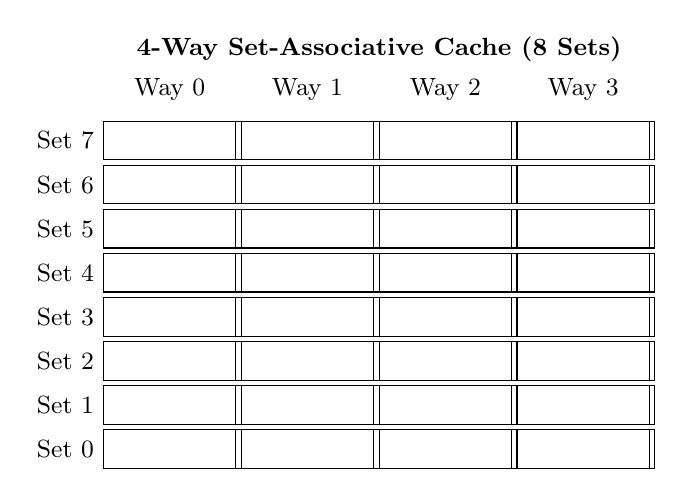
\begin{tikzpicture}[scale=0.7, every node/.style={font=\small}]
    % Draw sets
    \foreach \i in {0,...,7} {
        \draw (0,\i*0.8) rectangle (10,\i*0.8+0.7);
        \node[left] at (0,\i*0.8+0.35) {Set \i};
        
        % Draw 4 ways
        \foreach \j in {0,...,3} {
            \draw (\j*2.5,\i*0.8) rectangle (\j*2.5+2.4,\i*0.8+0.7);
        }
    }
    
    % Labels
    \node[above] at (1.2,6.5) {Way 0};
    \node[above] at (3.7,6.5) {Way 1};
    \node[above] at (6.2,6.5) {Way 2};
    \node[above] at (8.7,6.5) {Way 3};
    
    % Title
    \node[above] at (5,7.2) {\textbf{4-Way Set-Associative Cache (8 Sets)}};
\end{tikzpicture}
\caption{Cache Organization: 8 Sets $\times$ 4 Ways}
\end{figure}

\subsection{Cache Line Structure}

Each cache line contains:

\begin{table}[H]
\centering
\caption{Cache Line Components}
\begin{tabular}{@{}llp{7cm}@{}}
\toprule
\textbf{Field} & \textbf{Width} & \textbf{Description} \\
\midrule
Valid Bit & 1 bit & Indicates if line contains valid data \\
Dirty Bit & 1 bit & Indicates if line was modified (needs write-back) \\
Tag & 12 bits & Upper address bits for matching \\
Data & 256 bits & 32 bytes of cached data (8 words) \\
\bottomrule
\end{tabular}
\end{table}

%==============================================================================
\section{Interface Specification}
%==============================================================================

\subsection{CPU Interface}

The cache provides a simple CPU interface with three primary input signals as specified:

\begin{table}[H]
\centering
\caption{CPU-to-Cache Interface Signals}
\begin{tabular}{@{}llp{6cm}@{}}
\toprule
\textbf{Signal} & \textbf{Width} & \textbf{Description} \\
\midrule
\multicolumn{3}{l}{\textit{CPU $\rightarrow$ Cache (Inputs)}} \\
\midrule
cpu\_req\_valid & 1 & Request valid signal \\
cpu\_req\_addr & 20 & Memory address \\
cpu\_req\_rw & 1 & Read (0) / Write (1) \\
cpu\_req\_size & 2 & 00=byte, 01=half, 10=word \\
cpu\_req\_wdata & 32 & Write data from CPU \\
\midrule
\multicolumn{3}{l}{\textit{Cache $\rightarrow$ CPU (Outputs)}} \\
\midrule
cpu\_req\_ready & 1 & Cache ready for request \\
cpu\_resp\_valid & 1 & Response valid \\
cpu\_resp\_hit & 1 & Hit/miss indicator \\
cpu\_resp\_rdata & 32 & Read data to CPU \\
\bottomrule
\end{tabular}
\end{table}

\subsection{Memory Interface}

The cache communicates with main memory using line-based transfers:

\begin{table}[H]
\centering
\caption{Cache-to-Memory Interface Signals}
\begin{tabular}{@{}llp{6cm}@{}}
\toprule
\textbf{Signal} & \textbf{Width} & \textbf{Description} \\
\midrule
\multicolumn{3}{l}{\textit{Cache $\rightarrow$ Memory (Outputs)}} \\
\midrule
mem\_req\_valid & 1 & Memory request valid \\
mem\_req\_addr & 15 & Line/block address \\
mem\_req\_rw & 1 & Read (0) / Write-back (1) \\
mem\_req\_wdata & 256 & Line data for write-back (32 bytes) \\
\midrule
\multicolumn{3}{l}{\textit{Memory $\rightarrow$ Cache (Inputs)}} \\
\midrule
mem\_resp\_valid & 1 & Memory response valid \\
mem\_resp\_rdata & 256 & Line data from memory (32 bytes) \\
\bottomrule
\end{tabular}
\end{table}

%==============================================================================
\section{Functional Description}
%==============================================================================

\subsection{Cache Hit Operation}

On a cache hit:
\begin{enumerate}
    \item CPU presents address and request type
    \item Cache decodes set index and tag
    \item Parallel comparison of tag with all 4 ways
    \item On match with valid bit set: HIT
    \item For read: return requested word/half/byte
    \item For write: update data, set dirty bit
    \item Response in \textbf{1 clock cycle}
\end{enumerate}

\subsection{Cache Miss Operation}

On a cache miss:
\begin{enumerate}
    \item No tag match found in the set
    \item MSHR allocated with miss information
    \item Random victim selected using LFSR
    \item If victim is dirty: initiate write-back
    \item Request new line from memory
    \item On memory response: install line, complete request
    \item Response after \textbf{memory latency + overhead}
\end{enumerate}

\subsection{Random Replacement Policy}

The replacement policy uses a 16-bit Linear Feedback Shift Register (LFSR):

\begin{lstlisting}[style=verilog]
// LFSR update (polynomial: x^16 + x^14 + x^13 + x^11 + 1)
lfsr <= {lfsr[14:0], lfsr[15] ^ lfsr[13] ^ lfsr[12] ^ lfsr[10]};

// Victim selection (use 2 LSBs for 4-way)
victim_way = lfsr[1:0];
\end{lstlisting}

The LFSR provides pseudo-random victim selection with a period of $2^{16}-1 = 65535$.

\subsection{Write-Back Policy}

The cache implements write-back (copy-back) policy:

\begin{itemize}
    \item Writes only update the cache (not memory)
    \item Dirty bit tracks modified lines
    \item On eviction: if dirty, write line to memory first
    \item Reduces memory traffic for write-heavy workloads
\end{itemize}

\subsection{Non-Blocking with MSHR}

The Miss Status Holding Register (MSHR) enables non-blocking operation:

\begin{figure}[H]
\centering
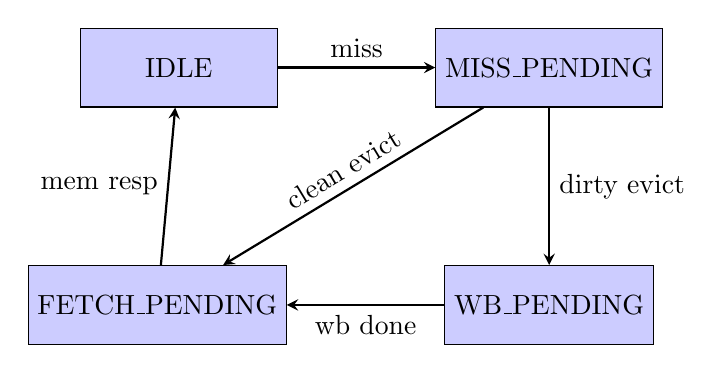
\begin{tikzpicture}[node distance=2cm, auto,
    state/.style={rectangle, draw, fill=blue!20, minimum width=2.5cm, minimum height=1cm},
    arrow/.style={->, >=stealth, thick}]
    
    \node[state] (idle) {IDLE};
    \node[state, right=of idle] (miss) {MISS\_PENDING};
    \node[state, below=of miss] (wb) {WB\_PENDING};
    \node[state, left=of wb] (fetch) {FETCH\_PENDING};
    
    \draw[arrow] (idle) -- node[above] {miss} (miss);
    \draw[arrow] (miss) -- node[right] {dirty evict} (wb);
    \draw[arrow] (wb) -- node[below] {wb done} (fetch);
    \draw[arrow] (miss) -- node[above,sloped] {clean evict} (fetch);
    \draw[arrow] (fetch) -- node[left] {mem resp} (idle);
\end{tikzpicture}
\caption{MSHR State Machine}
\end{figure}

MSHR fields stored during miss:
\begin{itemize}
    \item \texttt{mshr\_valid}: MSHR active flag
    \item \texttt{mshr\_block}: Requested block address
    \item \texttt{mshr\_set}: Target set index
    \item \texttt{mshr\_word}: Word offset within line
    \item \texttt{mshr\_rw}: Read/write type
    \item \texttt{mshr\_size}: Access size
    \item \texttt{mshr\_wdata}: Write data (for write miss)
    \item \texttt{mshr\_victim}: Selected victim way
    \item \texttt{mshr\_wb\_pending}: Write-back in progress
\end{itemize}

%==============================================================================
\section{Simulation Results}
%==============================================================================

\subsection{Test Overview}

The testbench verifies all cache functionality through 8 comprehensive tests:

\begin{table}[H]
\centering
\caption{Testbench Test Cases}
\begin{tabular}{@{}clp{6cm}@{}}
\toprule
\textbf{Test} & \textbf{Name} & \textbf{Purpose} \\
\midrule
1 & Hit Latency & Verify 1-cycle hit, measure miss penalty \\
2 & Data Sizes & Test byte, half-word, word access \\
3 & Conflict Misses & Demonstrate set associativity limits \\
4 & Write-Back & Verify dirty line eviction \\
5 & Sequential Access & Measure spatial locality benefits \\
6 & Write-Read & Verify write then read correctness \\
7 & Thrashing & Worst-case conflict pattern \\
8 & Non-Blocking & MSHR behavior verification \\
\bottomrule
\end{tabular}
\end{table}

\subsection{Performance Metrics}

\begin{table}[H]
\centering
\caption{Measured Performance}
\begin{tabular}{@{}ll@{}}
\toprule
\textbf{Metric} & \textbf{Value} \\
\midrule
Cache Hit Latency & 1 cycle \\
Cache Miss Penalty & $\sim$56 cycles (50 cycle memory + overhead) \\
Sequential Access Hit Rate & 87\% \\
Thrashing Hit Rate & 40\% \\
\bottomrule
\end{tabular}
\end{table}

\subsection{Conflict Miss Demonstration}

Test 3 demonstrates conflict misses by accessing 5 blocks that map to the same set:

\begin{verbatim}
Addresses mapping to Set 0: 0x000, 0x100, 0x200, 0x300, 0x400
(all have bits [7:5] = 000)

Phase 1: Fill 4 ways → 4 misses (cold misses)
Phase 2: Access 5th block → 1 miss (conflict, causes eviction)
Phase 3: Re-access evicted → miss or hit (random victim)

Statistics: This demonstrates limited associativity causing evictions
\end{verbatim}

\subsection{Write-Back Verification}

Test 4 verifies write-back by:
\begin{enumerate}
    \item Writing data to create dirty line
    \item Forcing eviction by filling the set
    \item Observing \texttt{WRITE(WB)} in memory log
\end{enumerate}

Sample output:
\begin{verbatim}
[CPU] Write addr=0x01000 data=0xDEADBEEF
  Result: MISS (line is now DIRTY)
[CPU] Read addr=0x01400 (force eviction)
    [MEM] Request: addr=0x00080 rw=WRITE(WB)  <-- Write-back!
    [MEM] Writeback complete
\end{verbatim}

%==============================================================================
\section{Implementation Details}
%==============================================================================

\subsection{Storage Arrays}

\begin{lstlisting}[style=verilog]
// Storage arrays (all lines stored linearly)
reg [TAG_BITS-1:0]  tag_array   [0:NUM_LINES-1];  // 32 x 12 bits
reg                 valid_array [0:NUM_LINES-1];  // 32 x 1 bit
reg                 dirty_array [0:NUM_LINES-1];  // 32 x 1 bit
reg [LINE_BITS-1:0] data_array  [0:NUM_LINES-1];  // 32 x 256 bits
\end{lstlisting}

\subsection{Hit Detection}

\begin{lstlisting}[style=verilog]
// Parallel tag comparison for all 4 ways
hit = 0;
base = addr_set * ASSOC;
for (way = 0; way < ASSOC; way = way + 1) begin
    idx = base + way;
    if (valid_array[idx] && tag_array[idx] == addr_tag) begin
        hit = 1;
        hit_idx = idx;
    end
end
\end{lstlisting}

\subsection{Data Size Handling}

\begin{lstlisting}[style=verilog]
// Write with size handling
bpos = addr_word * 4;  // Byte position
case (cpu_req_size)
    2'b00: line[bpos*8 +: 8]  = wdata[7:0];   // Byte
    2'b01: line[bpos*8 +: 16] = wdata[15:0];  // Half-word
    default: line[bpos*8 +: 32] = wdata;      // Word
endcase
\end{lstlisting}

%==============================================================================
\section{Scalability}
%==============================================================================

The cache design supports easy scaling by changing parameters:

\begin{table}[H]
\centering
\caption{Scaling Configurations}
\begin{tabular}{@{}cccccc@{}}
\toprule
\textbf{Size} & \textbf{Sets} & \textbf{SET\_BITS} & \textbf{TAG\_BITS} & \textbf{Lines} \\
\midrule
1 KB & 8 & 3 & 12 & 32 \\
2 KB & 16 & 4 & 11 & 64 \\
4 KB & 32 & 5 & 10 & 128 \\
8 KB & 64 & 6 & 9 & 256 \\
64 KB & 512 & 9 & 6 & 2048 \\
\bottomrule
\end{tabular}
\end{table}

To scale, modify these parameters in \texttt{cache.v}:
\begin{lstlisting}[style=verilog]
localparam NUM_SETS  = 8;    // Change: 8,16,32,64,512
localparam SET_BITS  = 3;    // Change: 3,4,5,6,9
localparam TAG_BITS  = 12;   // Change: 12,11,10,9,6
localparam NUM_LINES = 32;   // Change: 32,64,128,256,2048
\end{lstlisting}

%==============================================================================
\section{FPGA Implementation}
%==============================================================================

\subsection{Target Device}

\begin{table}[H]
\centering
\caption{FPGA Target Specifications}
\begin{tabular}{@{}ll@{}}
\toprule
\textbf{Parameter} & \textbf{Value} \\
\midrule
Board & DE0-Nano \\
FPGA & Cyclone IV EP4CE22F17C6 \\
Logic Elements & 22,320 \\
M9K Memory Blocks & 66 (594 Kbits) \\
Clock & 50 MHz \\
\bottomrule
\end{tabular}
\end{table}

\subsection{Synthesis Top Module}

The synthesis top module (\texttt{top\_synth.v}) provides:
\begin{itemize}
    \item Minimal I/O: clock, reset, 4 switches, 8 LEDs
    \item Internal memory stub with configurable latency
    \item Address pattern generator for testing
    \item Hit/miss counters displayed on LEDs
\end{itemize}

\subsection{Pin Mapping}

\begin{table}[H]
\centering
\caption{FPGA Pin Assignments}
\begin{tabular}{@{}lll@{}}
\toprule
\textbf{Signal} & \textbf{Direction} & \textbf{Function} \\
\midrule
clk\_50 & Input & 50 MHz clock \\
rst\_n & Input & Active-low reset \\
sw[3:0] & Input & Test pattern selection \\
led[7:0] & Output & Status and counters \\
\bottomrule
\end{tabular}
\end{table}

%==============================================================================
\section{Conclusion}
%==============================================================================

This project successfully implements a 4-way set-associative cache with the following achievements:

\begin{enumerate}
    \item \textbf{Architectural Correctness}: Proper set-associative organization with parallel tag comparison and correct address decoding.
    
    \item \textbf{Functional Correctness}: All operations (read hit, read miss, write hit, write miss, write-back) verified through comprehensive simulation.
    
    \item \textbf{Conflict Miss Demonstration}: Successfully shows cache thrashing when working set exceeds associativity.
    
    \item \textbf{Non-Blocking Operation}: MSHR correctly handles outstanding misses with proper state machine transitions.
    
    \item \textbf{Write-Back Policy}: Dirty bit tracking and write-back on eviction verified.
    
    \item \textbf{Scalable Design}: Parameters allow easy scaling from 1KB to 64KB.
\end{enumerate}

\subsection{Future Improvements}

Potential enhancements:
\begin{itemize}
    \item Multiple MSHRs for true non-blocking behavior
    \item LRU replacement policy option
    \item Prefetching support
    \item Multi-level cache hierarchy
    \item AXI or Wishbone bus interface
\end{itemize}

%==============================================================================
\appendix
\section{File Structure}
%==============================================================================

\begin{verbatim}
Set-Associative-Cache/
├── verilog/
│   ├── cache.v          # Main cache module
│   ├── top_synth.v      # FPGA synthesis top
│   └── tb_cache.v       # Testbench
├── Cache.qpf            # Quartus project file
├── Cache.qsf            # Quartus settings file
└── report/
    └── cache_report.tex # This report
\end{verbatim}

\section{Running Simulation}
%==============================================================================

To run the testbench using Icarus Verilog:

\begin{verbatim}
cd verilog
iverilog -o cache_sim cache.v tb_cache.v
vvp cache_sim
\end{verbatim}

To view waveforms:
\begin{verbatim}
gtkwave cache_sim.vcd
\end{verbatim}

\end{document}
